%!TEX root = ../thesis_a4.tex
\part{Knowledge-based Approaches}
\label{part:knowledge-based}

\chapter{Linking Texts to Music Knowledge Bases}
\label{sec:background}


\section{Introduction}

%%%%%%%%%%%%% LUIS CamReady %%%%%%%%%%%%%

When we refer to the Music Domain in a Natural Language Processing (NLP) context we refer to Music product reviews such as Albums or Songs, Music-related biographies or even song lyrics. While these are valuable resources in NLP for tasks like Sentiment Analysis, Music Information Retrieval (MIR), however, has barely exploited the information and knowledge that can be extracted from textual data. This opens up a vibrant area of research where MIR tasks may benefit dramatically from mining textual data \cite{Sordo2015}. 

Named Entity Recognition (NER) is the task to identify mentions to entities belonging to a set of predefined categories \cite{ZhouandJian2002}. Traditionally, the most widely covered types of entities are \textsc{Person}, \textsc{Location} and \textsc{Organization}, as well as numeric expressions or time-spans. While NER is a widely studied topic, and has been at the core of well-known shared tasks and conferences \cite{Nadeau2007} such as MUC, ACE or CoNLL, the advent of large knowledge repositories and collaborative resources has contributed to the emergence of another discipline: Entity Linking (EL), i.e. to discover mentions of entities in text and link them to a suitable knowledge repository \cite{Moroetal2014}.


to obtain an annotation for Music entity mentions in text, either simply as Music types (e.g. tagging `Yellow Submarine' as \texttt{Song}) or performing Entity Linking (EL), e.g. tagging `Yellow Submarine' as \texttt{dbpedia.org/page/Yellow\_Submarine\_(song)}. However, this is not a trivial task as mentions to Music entities show language and register idiosyncrasies \cite{TataandDiEugenio2010,Gruhl2009}, and therefore a certain degree of tailoring is required in order to account for them. Let us consider multiword Music entities, which usually are those who pose greatest challenges for EL. As \cite{TataandDiEugenio2010} point out, they are difficult to discover because they may not be restricted to a single Noun Phrase or may be abbreviated (by means of acronyms, dropping entire words or even full rephrasing). Additionally, a specific trait of Music texts is the fact that one song may have many covers by many different artists and, according to our evaluation, it may be difficult even for a human to identify what \textit{version} of the song the writer is referring to. Furthermore, availability of EL testbeds in general \cite{Usbeck2015}, and in the Music domain in particular \cite{Gruhl2009}, is scarce, making it very difficult to evaluate novel systems and approaches. Hence, it is difficult to know how well a certain method, which may work well for generic texts, will perform on Music data.

%The advent of large Knowledge Repositories or Knowledge Bases (KBs) and collaborative resources has contributed to the emergence of Entity Linking (EL), 
%%%i.e. the task of discovering mentions of entities in text and link them to a suitable KB \cite{Moroetal2014}. 
%In the context of Open Data, there is an increasing need for benchmarking and evaluation corpora. However, while general purpose datasets exist , dealing with highly specific domains (e.g. chemistry) or ever-evolving areas (e.g. videogames or music) poses a greater challenge for EL due to linguistic idiosyncrasies or under-representation in general purpose KBs. The latter is precisely the case of the music domain , where available evaluation data for EL is scarce.

Despite the current context of scarcity of both EL systems and evaluation benchmarks in the Music domain, there are some exceptional cases in which these issues were addressed, such as: (1) Detecting Music entities (e.g. songs or bands) on informal text \cite{Gruhl2009}; (2) Applying Hidden Markov Models for discovering Music entity mentions in Chinese corpora \cite{Zhang2009}; or (3) Recognizing musical entities in the context of a relation extraction pipeline \cite{Oramas2015}. 

We argue that the problem of precision in detecting musical entities may be tackled by leveraging a combination of several generic EL off-the-shelf systems. Simply put, we hypothesize that if two or more generic systems annotate with the same URI an entity mention, the probability of this annotation to be correct increases. To the best of our knowledge, very little effort has been put in exploiting this \textit{agreement} feature. One of the reasons may be that, as of now, most EL systems \textit{speak their own language}, partially due to the fact that each of them points back to different KBs, and hence their output is heterogeneous and cannot be directly compared, let alone combine. This has motivated research towards unification frameworks for evaluation of EL. For instance, \cite{Cornolti2013} put forward a benchmarking framework for comparing EL systems. Moreover, \cite{Rizzo2014} describe a system aimed at combining the output of the different NER systems. Finally \cite{Usbeck2015} present \textsc{GERBIL}, an evaluation framework for semantic EL based on \cite{Cornolti2013}. %This is an open-source and extensible framework that allows evaluating tools against different datasets.

%%%cornolti2013 -> , leveraging Wikipedia, and a hierarchy of EL problems. 
%%%rizzo2014 -> %divide the process into NER and EL, evaluating each stage individually. They subsequently 

In this chapter we aim to provide a twofold answer to the challenges described above, and bridge the gap between the Music domain and EL. Specifically, we present \textsc{ELMD}, an automatically constructed corpus where named entities are classified as any of four predefined \textit{musical categories}, namely \textsc{Song}, \textsc{Album}, \textsc{Artist}, and \textsc{Record Label}, by leveraging the hyperlinks present in a set of artist biographies. Then, we further enrich \textsc{ELMD} by performing EL and automatically annotating a large portion of the entities with their \textsc{DBpedia} URI. The source data used in this paper comes from the music website and social network Last.fm\footnote{http://www.last.fm}. To the best of our knowledge, this is the first attempt to provide an annotated large-scale 
%crowdsourced (i.e. without corporate bias) 
corpus of linked entities in the music domain. % as Linked Data.
Finally, a subset of 200 documents from ELMD is manually annotated to provide a comprenhensive dataset of annotated documents. This latter dataset have been uses in the context of the 3rd Open Knowledge Extraction Challenge \cite{TODO}.

%\textsc{ELMD} is built by leveraging hyperlinks appearing in artist biographies collaboratively written by the Last.fm community, together with the integration of three state-of-the art EL systems. In this way, we produce a highly precise mapping between a Last.fm URL and its corresponding \textsc{DBpedia} URI. 

The final resource amounts to 47,254 sentences, in which 92,930 entities are categorized into the aforementioned \textit{musical categories}, and 64\% of them are disambiguated and linked to DBpedia. We achieve a Precision score of 97\% in the most restrictive setting, in which our approach manages to annotate more than 31,000 entities.

In the remainder of this paper, we first introduce \textsc{ELVIS} (Entity Linking Voting and Integration System), our EL integration and agreement approach. Then, we describe the text corpus we compiled from the \textsc{Last.fm} website and how it is combined with ELVIS. In the next step, the obtained dataset is evaluated. Finally, we describe the resulting output of our system: The \textsc{ELMD} dataset. 
%A summary of our approach is provided in Figure \ref{fig:workflow}.


\section{Music Knowledge Bases}\label{sec:related_work:mus_rec}

\textsc{MusicBrainz} and \textsc{Discogs} are two paramount examples of manually curated \textsc{MKBs}. They are open music encyclopedias of music metadata built collaboratively and openly available. \textsc{MusicBrainz}, in addition, is regularly published as Linked Data by the \textsc{LinkedBrainz} project\footnote{\url{http://linkedbrainz.org/}}.

As for generic \textsc{KBs} based on \textsc{Wikipedia}, such as the ones described earlier, these include a remarkable amount of music data, such as artist, album and song biographies, definitions of musical concepts and genres, or articles about music institutions and venues. However, their coverage is biased towards the best known artists, and towards products from Western culture. Finally, let us refer to the notable case of \textsc{Grove Music Online}\footnote{\url{http://www.oxfordmusiconline.com}}, a music encyclopedia containing over 60k articles written by music scholars. However, it has the drawback of not being freely open, as it runs by subscription.

Other than the aforementioned curated repositories, to the best of our knowledge, there is not a single automatically learned open \textsc{MKB}. A first step in this direction was taken in \cite{Sordo2015,Oramas2014}, applying \textsc{RE} techniques to big datasets of music related texts extracted from the web. Moreover, in \cite{Oramas2015b}, a Flamenco \textsc{MKB} is created by combining data from curated \textsc{KBs} and information extracted from blogs and websites.

Despite their scarcity, \textsc{MKBs} are becoming increasingly popular in MIR applications, such as artist similarity and music recommendation \cite{Celma2008,Oramas2015a,Leal2012,Ostuni2015}. 
MKBs have also been exploited as sources of explanations in music recommender systems. According to~\cite{CelmaandHerrera2008}, giving explanations of the recommendations provides transparency to the recommendation process and increases the confidence of the user in the system. In \cite{Passant2010}, explanations of recommendations are created by exploiting \textsc{DBpedia}'s structured information, whilst in \cite{Sordo2015}, explanations are based on an automatically learned \textsc{MKB}. 



\section{ELVIS}
\label{sec:method}

In this section we describe \textsc{ELVIS}, the generic integration framework for Entity Linking, which is leveraged for the construction of \textsc{ELMD}. First, we describe our Entity Linking research problem and provide an intuition on how this may be surmounted via an agreement scheme. Then, we provide details on the main modules integrating \textsc{ELVIS}, highlighting the possible cases of agreement and disagreement over the EL systems that are integrated in our framework.

\subsection{Argumentum ad Populum in EL}
\label{sec:tools}

Our method relies on the \textit{argumentum ad populum} intuition, i.e. if two or more different EL systems perform the same prediction in linking a named entity mention to its entry in a reference KB, the more likely this prediction is to be correct. We put this intuition into practice by combining the output of three well-known systems, namely DBpedia Spotlight~\cite{Mendes2011} , Tagme~\cite{Ferragina2012} and Babelfy~\cite{Moroetal2014b}, whose agreement (or disagreement) when disambiguating an in-text entity mention is taken as an agreement-driven \textit{confidence score}. These specific tools were chosen for being considered state-of-the-art EL systems and for being well known in the NLP community. However, \textsc{ELVIS} can easily incorporate any additional system. We also selected these tools because entities identified by all of them can be easily referenced to DBpedia URIs. Although there are other knowledge bases (e.g. MusicBrainz) with substantially more musical entities than DBpedia, to the best of our knowledge, there is no EL tool that works with these domain specific knowledge bases. 

Let us briefly describe each of the selected EL systems:
\begin{itemize}
\item \textbf{DBpedia Spotlight} \cite{Mendes2011} is a system for automatically annotating text documents with DBpedia URIs, finding and disambiguating natural language mentions of DBpedia resources. DBpedia Spotlight is shared as open source and deployed as a Web service freely available for public use\footnote{https://github.com/dbpedia-spotlight}.
DBpedia Spotlight gives as a result the DBpedia URI, start and end char positions, the value of the rdf:type property, and a confidence score for for each prediction.
\item \textbf{TagMe} \cite{Ferragina2012} is an EL system that matches terms with Wikipedia link texts and disambiguates them using the in-link graph and the Wikipedia page dataset. Then, it performs a pruning process by looking at the entity context. TagMe is available as a web service\footnote{http://tagme.di.unipi.it/}, and provides the Wikipedia page id, Wikipedia categories, and a confidence score. 
\item \textbf{Babelfy} \cite{Moroetal2014b} is an EL and Word Sense Disambiguation based on non-strict identification of candidate meanings (i.e. not necessarily exact string matching), together with a graph based algorithm that traverses the BabelNet graph and selects the most appropriate semantic interpretation for each candidate. Babelfy is available as a web service\footnote{http://babelfy.org/guide}. Its output is based on the corresponding BabelNet synset of the disambiguated mention. If the synset references to a Wikipedia page, it returns the Wikipedia URL, the DBpedia URI, as well as Wikipedia categories.
\end{itemize}

While these tools have proven highly competitive on their own, in this paper we explore the gain in performance obtained by combining them together, and apply global agreement-driven decisions on the \textsc{Last.fm} corpus.
%, which we describe next.

%Integrating any number of EL tools is not a trivial task, as they have their own unique way of representing annotated entities (e.g. character vs. word offset, or reference KB used). In what follows, we describe experiments carried out on the Last.fm text corpus (described in Section \ref{lastfmcorpus}). We specifically tackle the problem of integrating the above EL tools (Section \ref{unification}). Finally, this integration allows us to introduce an agreement-based measure (Section \ref{agreement}), which we evaluate extensively on a sample of 1700 sentences (Section \ref{evaluation}).

%We explain how we surmount this problem in Section \ref{unification}. Once the unified framework is achieved, we apply an agreement-based approach to the Last.fm text corpus (Section \ref{lastfmcorpus} using an agreement-based approach (Section \cite{agreement}). Finally, we evaluate the quality of the linked entities and, consequently. the soundness of our approach, over a sample of 1700 sentences (Section \cite{evaluation}).

\subsection{`Translating' EL Formats}
\label{sec:unification}

In order to have each EL system \textit{speak the same language} for measuring agreement in their predictions, output homogenization is required. This is not a trivial task, as each EL approach may be based on a different reference KB, the offsets may be computed differently, and so on. For instance, DBpedia Spotlight links entity mentions via DBpedia URIs, whereas Tagme provides Wikipedia page IDs, and Babelfy disambiguates against BabelNet \cite{NavigliPonzetto2012} and its corresponding BabelNet synsets. 
%Thus, we aim at exploiting the simple but powerful intuition that the more an arbitrary number of EL systems agree in their decision when disambiguating a named entity, the more likely this decision is to be correct. We therefore propose an agreement-based approach and apply it to the raw Last.fm corpus.
%Since our agreement-based approach requires a homogenization of the outputs, 
We attempt to surmount this heterogeneity as follows: First, we retrieve DBpedia URIs of every named entity. There are some considerations to be taken into account, however: (1) Character encoding differs from system to system, which we address by converting the character encoding of the retrieved URI to \textsc{UTF-8}; (2) Several URIs may refer to the same DBpedia resource. We solve this specific issue thanks to the transitive redirections provided by DBpedia. If a URI has a transitive redirection, it is replaced by the redirected URI. (3) Note that, in the case of Tagme, only Wikipedia page IDs are provided, which we can straightforwardly exploit to map entity mentions to their DBpedia equivalent. Finally, and after surmounting compatibility issues among systems, we retrieve DBpedia types (\texttt{rdf:type property}) for all entities. This \textit{type} information is further used in the creation of \textsc{ELMD}.
%The source code of this EL unification framework is released as open source.

%and quotation -> "character encoding AND QUOTATION(?)"

%\subsection{EL Agreement}
%\label{sec:agreement}

After successfully providing a process which harmonizes the output of EL systems, it is possible to compute the degree of agreement among them, which will become our system's confidence score. We define the following set of \textit{agreement heuristics} to set such score for each linking prediction (an overview of the workflow of \textsc{ELVIS} is provided in Figure \ref{fig:workflow}).

\begin{itemize}
    \item \textbf{Full Agreement $(++)$} When all systems detect an entity with the same URI and offset.
    \item \textbf{Partial Agreement $(+)$} When more than one but less than all systems detect an entity with the same URI and offset. Outliers (i.e. systems performing a different prediction) may detect a different entity or may not detect anything.
    \item \textbf{Singleton Decision $(-)$} When only one system detects an entity for a given text offset.
    \item \textbf{Disagreement $(--)$} When more than one system performs a linking over the same text offset, but all of their predictions are different.
\end{itemize}

%If all the three systems detect an entity with the same URI and offset, our system's confidence is 3, whereas confidence is set to 2 when only two of them agree (the remaining system may not detect anything or detect a different entity). However, if only one system detects an entity in a given text snippet, our confidence score is 1 (we refer to these entities as \textit{singletons}). Finally, we classify as \textit{disagreement} those cases where more than one system detects something in a given snippet but there is no agreement. 
%%%The output of the agreement step follows the same data structure as the output of the unification step, but adding to every entity the confidence score and the name of the tool or tools involved in the agreement. In case of disagreement, the different URIs and DBpedia types from every tool are provided.


\begin{figure}[h!]
  \centering
	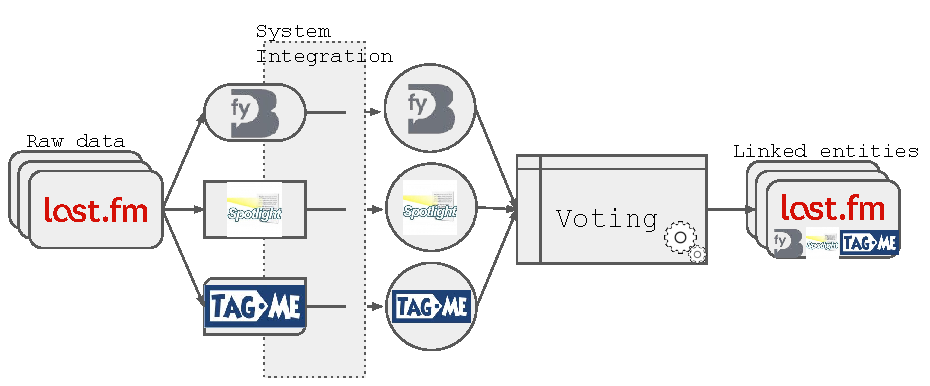
\includegraphics[height=3.25cm,width=8cm]{ch03_background/pics/workflow.pdf}
  \caption{ELVIS Workflow}
  \label{fig:workflow}
\end{figure}


\section{From \textsc{Last.fm} to \textsc{ELMD}}
\label{sec:lastfmcorpus}

In what follows, we describe the original data gathered from \textsc{Last.fm}, and the process to apply the integration framework described in Section \ref{sec:method}, in order to construct a highly precise benchmarking dataset for EL in the Music domain.


In \textsc{Last.fm}, users may add relevant biographical details to any artist's main page in the form of a \textit{wiki}. These edits are regularly moderated. Furthermore, artist biographies are often enriched with hyperlinks to other \textsc{Last.fm} Artist, Album, Song and Record Label pages, similarly as with Wikipedia hyperlinks. Our purpose is to leverage this meta-information to automatically construct a dataset of Music-specific annotated named entities.% and for evalauting the soundness of \textsc{ELVIS}.\\

We crawled artist biographies from \textsc{Last.fm} in March 2015, and gathered 13,000 artist biographies, which comprise 47,254 sentences with at least one hyperlink, amounting to a total of 92,930 links. These may be broken down as follows: (1) 64,873 hyperlinks referencing Artist pages; (2) 16,302 to Albums; (3) 8,275 to Song pages; and finally (4) 3,480 hyperlinks referencing Record Labels. This \textit{type} information is extracted thanks to the structure of each link's URL, as it includes in its path the category of the annotated entity. Consider, for example, the following sentence:

\begin{adjustwidth}{2.5em}{20pt}
\begin{center}
After their debut The Intelligence got signed to \textit{In the Red Records}.\\
\end{center}
\end{adjustwidth}


Here, we may infer that the entity \textit{In the Red Records} is a Record Label, thanks to its \textsc{Last.fm} URL: {\footnotesize{\texttt{http://www.last.fm/{\normalsize\textbf{label}}/In+the+Red+Records}}}. This information is extracted from the whole \textsc{Last.fm} corpus for those entities falling in one of the four \textit{musical categories} previously defined.

%%%\begin{figure}[h!]
%%%  \centering
%%%	\includegraphics[height=3.5cm]{elmd_creator.png}
%%%  \caption{Dataset creation.}
%%% \label{fig:dataset_creator}
%%%\end{figure}

%After this extraction process, a first version of the dataset is built with the identified and categorized named entities.



\subsection{Data Enrichment}

For the creation of the ELMD dataset, the crowdsourced annotations extracted from \textsc{Last.fm} biographies are combined with decisions made by \textsc{ELVIS} and its voting framework.\\%(see Figure~\ref{fig:dataset_creator}).

Every entity mention annotated in the \textsc{Last.fm} corpus is a candidate to be included in \textsc{ELMD}. The challenge is to assign to each entity its correct DBpedia URI. We approach this problem by leveraging (1) The DBpedia URI assigned by \textsc{ELVIS}, (2) The \textit{agreement score} for that prediction, as well as (3) The \textit{type} information derived from the entity's \textsc{Last.fm} URL. Our intuition is that the higher the \textit{agreement score}, the more likely the prediction is to be correct. Likewise, we also hypothesize that if a linking decision made by \textsc{ELVIS} coincides in \textit{type} with the original \textsc{Last.fm} annotation, it is more likely to be correct. Since there is no direct mapping between \textsc{Last.fm} and DBpedia types, we manually set the type equivalences shown in Table \ref{tbl:equivalence}.\\

Regarding the \textit{agreement score}, it corresponds to the number of systems that agreed in a decision (see \textbf{Score} column in Table \ref{tbl:examples}). Note that an \textit{agreement score} of 1 may be caused either by cases in which only one system detected an entity mention, or when there is disagreement among systems, but one and only one of them coincides in \textit{type} with the original \textsc{Last.fm} annotation (last row in Table \ref{tbl:examples}).

As for \textit{type value}, this is a binary value (\textit{type-equivalent} or \textit{type-discrepant}) based on coinciding types between \textsc{Last.fm} URLs and \textsc{ELVIS} decisions.
%Note that agreement across systems within \textsc{ELVIS} is not considered (for instance, systems in \textsc{ELVIS} coincide in the example given in the third row of Table \ref{tbl:examples}, but its \textit{type value} is set to \texttt{discrepant} since it does not match with the entity's \textsc{Last.fm} type).

%Additionally, when an entity is considered as disagreement by the agreement framework, but there is type equivalence with  one of the three EL systems, we change its confidence score from 0 to 1, and consider it also as a \textit{singleton} (there is an example of this special case in last row of Table~\ref{tbl:examples}).\\

%To measure the usefulness of the type information, we divide the evaluation in two settings namely: (1) \textit{Type equivalence}, when the predicted and target entities share an equivalent type; and (2) \textit{Type nonequivalence}, when this is not the case. Note that for \textit{type nonequivalence} we consider both cases in which Last.fm and DBpedia types do not coincide, or when type information is absent in the DBpedia resource. 

%added to the ELMD dataset along with two features, namely its corresponding offset and \textit{type} information. Then, \textsc{ELVIS} is used to provide a linking between these entities and DBpedia as follows: For each detected entity, if the offset of the \textsc{Last.fm} annotation and an \textsc{ELVIS} prediction coincide, we leverage the \textit{confidence score} provided by the agreement among systems integrating \textsc{ELVIS} together with the entity type (see Table \ref{tbl:equivalence}).% and use it as a confidence booster. %Therefore, there are two parameters that are used in the decision process, the confidence score and the type equivalence flag.


%provides a high precision linking between these entities and DBpedia. For each annotated entity, we obtain two important pieces of information: (1) \textsc{ELVIS} confidence score, which is obtained after applying the aforementioned \textit{agreement heuristics}; and (2) \textit{type} information, obtained from the original \textsc{Last.fm} data. 


%if there is an entity in the agreement output with the same offset, we analyze its confidence score and type information to decide whether to take its URI or not.
%We compare the type information gathered from DBpedia with the music categories inferred from the original Last.fm data 

%If our system considers both type information as equivalent, the 

%Additionally, in the type agreement setting, we consider as \textit{singleton} instead of disagreement, decisions cases in which 
%more than one system detects something in a text snippet, and they predict different entities, but 
%only one system predicts the correct type of the entity, giving to this entities a confidence score of 1.

%We acknowledge that, while this additional information may be helpful for enriching the Last.fm corpus, it does not reflect a realistic scenario in which we would perform EL on unseen data. 


%In addition to system agreements, we apply a music-specific heuristic exploiting music categories inferred from the original Last.fm data. Specifically, we use the \textit{music type} information provided through the rdf:type property of DBpedia resources as an agreement booster. This means that if the agreed URI contains a type that equivalent to the category of the candidate entity (see Table \ref{tbl:equivalence}), we consider this as a case of \textit{type agreement}. For every level of system agreement, we differentiate the cases where there is type agreement from the other cases. In addition, when there is disagreement between systems, but only one of them detects an entity with type agreement, our confidence score is 1, like for singletons.

\begin{table}[ht!]
\small
\centering
\def\arraystretch{1.2}
	\begin{tabular}{|l|l|}
\hline
\textbf{Last.fm type} & \textbf{DBpedia type} \\
\hline
Song & DBpedia:Song, DBpedia:Single, Yago:Song \\
Album & \parbox[t]{5cm}{DBpedia:Album, Yago:Album,\\ Schema:MusicAlbum} \\
Artist & \parbox[t]{5cm}{DBpedia:MusicalArtist, \\DBpedia:Band, Schema:MusicGroup, Yago:Musician, Yago:Creator, DBpedia:Artist} \\
Record Label & DBpedia:RecordLabel \\
\hline
	\end{tabular}
	\caption{Type equivalence}
	\label{tbl:equivalence}
\end{table}

\begin{table*}[!t]
%\scriptsize
\def\arraystretch{1.2}
\centering
	\begin{tabular}{| p{3cm} | c | p{2cm} | p{2cm} | p{2cm} | c | c |}
\hline
\textbf{Context} & \textbf{Last.fm type} & \textbf{Tagme} & \textbf{Babelfy} & \textbf{Spotlight} & \textbf{Score} & \textbf{Type Eq.} \\
\hline
and the academic minimalism of \textbf{Steve Reich} & Artist &  Steve\_Reich (type:artist) & Steve\_Reich (type:artist) & Steve\_Reich (type:artist) & 3 & \parbox[t]{2cm}{type-equivalent} \\
\hline
The new album \textbf{Hypocrisy} followed shortly thereafter & Album & --- & Hypocrisy (type:band) & Hypocrisy (type:band) & 2 & \parbox[t]{2cm}{type-discrepant} \\
\hline
The third album \textbf{Lucifer Songs}, opened new and unexpected doors & Album & --- & Lucifer\_Songs (type:album) & --- & 1 & \parbox[t]{2cm}{type-equivalent} \\
\hline
The band's debut album, \textbf{Cookies}, was released on 14 May 2007 & Album & HTTP\_cookie {\footnotesize{(type:unknown)}} & Cookies (type:album) & --- & 1 & \parbox[t]{2cm}{type-equivalent\\ (only\\ Babelfy)} \\
\hline
	\end{tabular}
	\caption{Agreement examples}
	\label{tbl:examples}
\end{table*}

%\subsection{Unification Framework for Entity Linking}

%\subsection{Agreement-based Entity Linking Confidence}

\begin{figure}[!t]
  \centering
	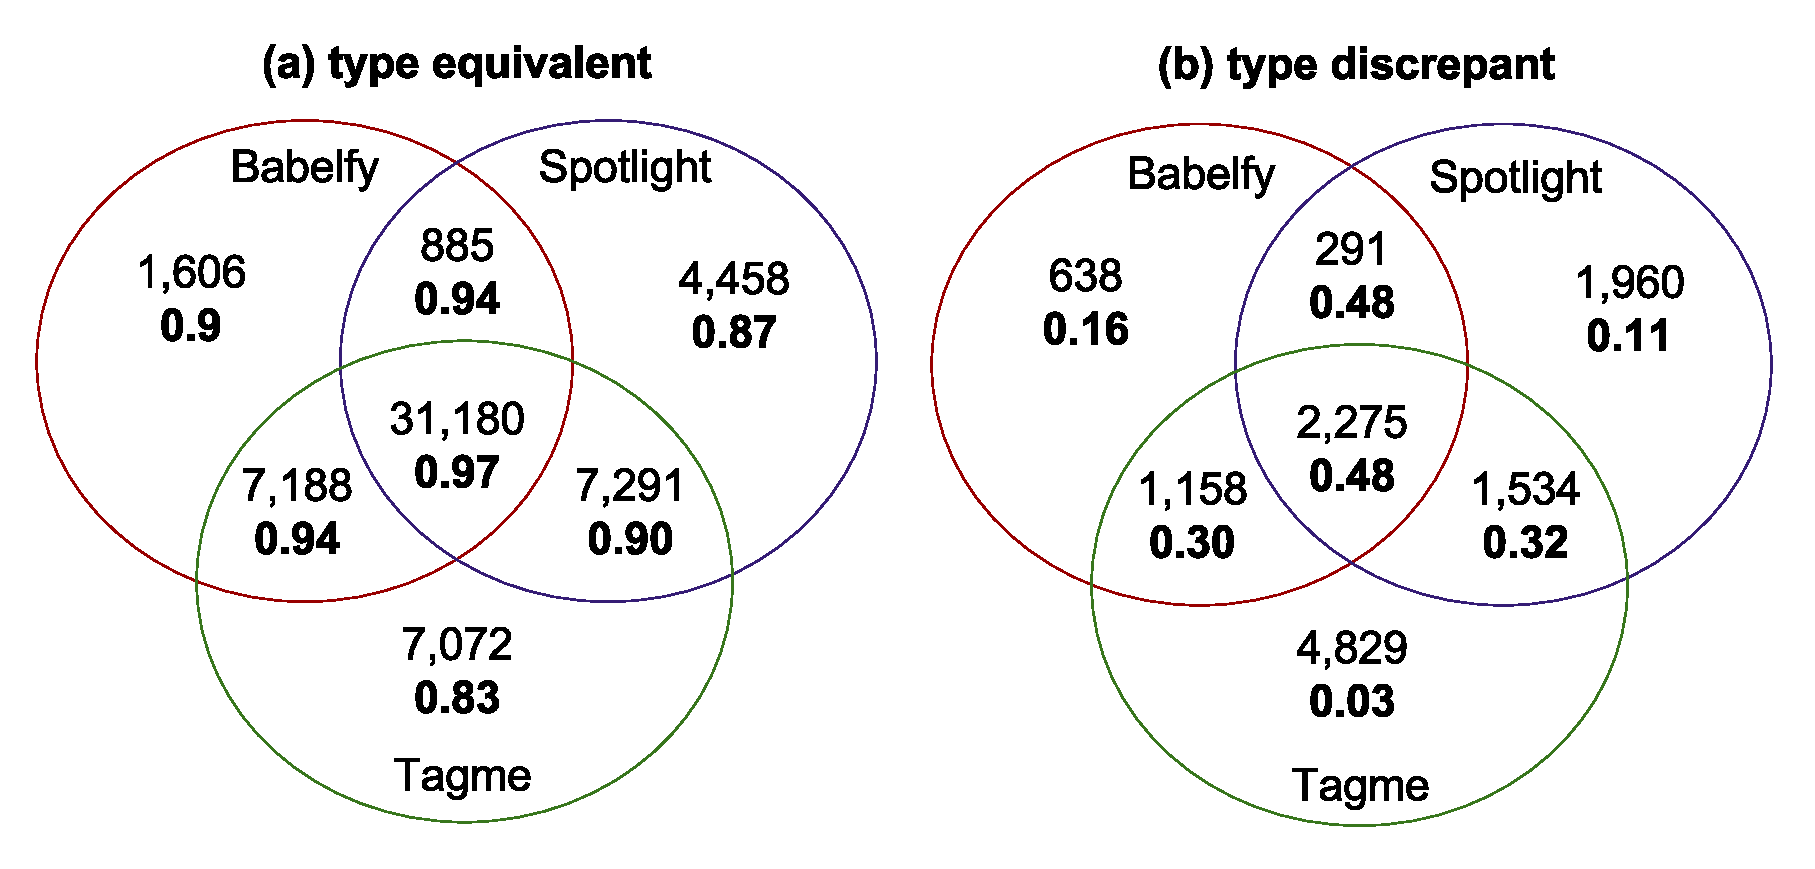
\includegraphics[width=8cm]{ch03_background/pics/evaluation_both.eps}
  \caption{Number of entities and precision of the manual evaluation.  Note the major differences in Precision between \textit{type-equivalent} and \textit{type-discrepant} systems.}
  \label{fig:agreement_typed}
\end{figure}

\begin{table}[ht!]
\centering
\def\arraystretch{1.2}
	\begin{tabular}{| c | c | c | c | c |}
\cline{2-4}
\multicolumn{1}{ c |  }{} & \textbf{Agreement} & \textbf{Precision} & \textbf{No. Entities} \\
\hline
\multirow{3}{*}{type-equivalent} & $=3$ & 0.97 & 31,180\\
&$\geq2$ & 0.96 & 46,544 \\
&$\geq1$ & 0.94 & 59,680 \\
\hline
%\multirow{3}{*}{type equivalence + type nonequivalence} & $=3$ & 0.94 & 33,455\\
\multirow{3}{*}{all} & $=3$ & 0.94 & 33,455\\
&$\geq2$ & 0.90 & 51,802\\
&$\geq1$ & 0.81 & 72.365\\
\hline
	\end{tabular}
	\caption{Precision and number of entities with this value of precision. \textit{Type-equivalent} implies entities from the type-equivalent configuration only, whilst \textit{All} implies all entities regardless their type information.}
	\label{tbl:results}
\end{table}

\section{Evaluation}
\label{evaluation}



Considering the different possibilities of agreement across the systems integrating \textsc{ELVIS}, there are in total 7 possible configurations: 1 with \textbf{full agreement} (score$=3$); 3 with \textbf{partial agreement} (score $=2$); and 3 \textbf{singleton} configurations (score$=1$). Moreover, considering also the two possible values of \textit{type agreement}, namely \texttt{equivalent} and \texttt{discrepant}, we have a total number of 14 configurations. Figure \ref{fig:agreement_typed} provides a visual overview of these configurations, where we show both Precision scores for each configuration (in bold) in addition to the number of entities disambiguated with \textsc{ELVIS} in each case.

%Considering the two possible values of \textit{type agreement}, namely \texttt{equivalent} and \texttt{discrepant}, and the different possibilities of agreement across the systems integrating \textsc{ELVIS}, there are in total 14 possible configurations. These may be broken down into 7 configurations with \textit{type equivalence} and 7 configurations with \textit{type discrepancy}. These 7 configurations according to EL agreement: 1 \textbf{full agreement} configuration (score$=3$); 3 \textbf{partial agreement} configurations (score $=2$); and 3 \textbf{singleton} configurations  (score$=1$). Figure \ref{fig:agreement_typed} provides a visual overview of these configurations, where we show both Precision scores for each configuration (in bold) in addition to the number of entities disambiguated with \textsc{ELVIS} in each case.\\
\begin{table*}[ht!]
\small
\centering
\def\arraystretch{1.2}
	\begin{tabular}{|l|r|r|r|l|}
\hline
\textbf{Musical Category} & \textbf{Annotations} & \textbf{Distinct Entities} & \textbf{Avg. words} & \textbf{Most frequent entity} \\
\hline
Song & 3,302 & 2,823 & 2.81 & Shine (6) \\
Album & 7,872 & 6,897 & 2.69 & Like Drawing Blood (6) \\
Artist & 46,337 & 17,535 & 1.88 & The Beatles (160) \\
Record Label & 2,169 & 815 & 1.94 & Sub Pop (33) \\
\hline
	\end{tabular}
	\caption{Statistics of the linked entities in ELMD. We report, for each \textit{musical category}, the total number of annotations linked to DBpedia, number of unique entities, average number of words per entity mention, and most frequently annotated entity (along with its frequency).}
	\label{tbl:statistics}
\end{table*}

%(1 with \textbf{full agreement} 3, 3 with \textbf{partial agreement}, and 3 with confidence 1) with \textit{type equivalence}, and 7 with \textit{type nonequivalence}. These 14 combinations are illustrated in Figure~\ref{fig:agreement_typed}. 

We evaluated 100 randomly selected entity samples (25 for each of the four Music categories we consider) from each one of the 14 possible configurations, and asked an eva\-luator with computational linguistics background to manually assess the correctness of the 1,400 predictions. From scores obtained from manual evaluation, we estimated Precision for the whole \textsc{ELMD} dataset with different ranges of \textit{agreement score} as well as two options \textit{type}-wise (see Table~\ref{tbl:results}). The precision value for all the entities is computed proportionally according to the number of entities and the precision obtained in the manual evaluation for the \textit{type-equivalent} and \textit{type-discrepant} settings, hence these can be seen as Micro Average Precision numbers.

We observe that the \textit{type-equivalent} configuration yields much better Precision with only a slight tradeoff in terms of Recall. Therefore, we decided to select for the final \textsc{ELMD} dataset only those URIs stemming from a \textit{type-equivalent} setting where \textit{agreement score} is equal or greater to 1. This ensures a Precision of at least 0,94 in terms of Entity Linking. Moreover, a manual survey of false positives in the highest scoring setting (\textit{agreement score}$=3$ and \textit{type-equivalent}) showed that these are cases in which even a human annotator may not find it trivial to correctly find the correct entity to those entity mentions. One of these cases are those in which \textsc{ELVIS} is presented with and entity mention that on surface may refer to either an Artist or an Album named after the artist or band itself. An actual case of false positive in our evaluation dataset is the following sentence:
\begin{adjustwidth}{2.5em}{20pt}
\begin{center}
Her debut album , \textit{Kim Wilde}, (released on RAK records) came out in July 1981 and stayed in the U.K. album charts for 14 weeks, peaking at number 3 and getting much acclaim.
\end{center}
\end{adjustwidth}

Here, the entity \textit{Kim Wilde} should be disambiguated as the Album with the same name as the artist, but \textsc{ELVIS} incorrectly assigned the Artist's DPpedia URI: {\footnotesize{\texttt{dbpedia.org/resource/Kim\_Wilde}}}. In \textsc{ELMD} there are 50 cases where the same surface text is correctly linked to an Artist entity in some sentences, and to a Song entity in others. Similar ambiguous cases involving Artist and Album (148) and Song and Album (95) are correctly resolved by our system. These particularly challenging cases may be interesting for training Music specific EL algorithms.

Another interesting source of false positives comes between musical entities and equally named entities (not necessarily related to Music). In cases in which the latter are more popular in a reference KB, e.g. their associated node in the graph may have higher connectivity, may become prioritized by disambiguation EL algorithms that consider graph connectivity as a feature. Consider the following sentence:

\begin{adjustwidth}{2.5em}{20pt}
\begin{center}
He is becoming more and more in demand for his remixing skills; working for the likes of Justin Timberlake and Armand van Helden, and labels including \textit{Ministry Of Sound}, Defected and Intec, to name a just a few.
\end{center}
\end{adjustwidth}

Here, the entity \textit{Ministry of Sound} refers to a Record Label, a spin-off of the well-known club, which is the entity that was incorrectly assigned: {\footnotesize{\texttt{dbpedia.org/resource/Ministry\_of\_Sound}}}. 
Cases like this would require, first, to ensure that the different entities derived from \textit{Ministry of Sound} (such as the Record Label or a clothing brand of the same name) exist in a reference KB, and second, to exploit contextual information so that a correct decision is made.
A similar situation happens when song or album names may be confused with very common words or expressions (e.g. `Easy', `Stupid', `Sad song', `If', `Be there'). \textsc{ELMD} is rich in challenging cases like these.

%It would be very difficult, even for human annotators to obtain higher Precision. %[EJEMPLO DE CASO CONCRETO]

%We randomly selected a sample of 100 entities from each one of the 14 sets of entities defined in Figures~\ref{fig:agreement_typed} and~\ref{fig:agreement_nontyped}. In Figure~\ref{fig:agreement_typed} are represented the entities with type agreement, whereas in Figure~\ref{fig:agreement_nontyped} are represented the ones where the condition of agreement was not satisfied, whether because there is disagreement between the Last.fm type and the DBpedia type, or because there is not enough type information in the DBpedia resource. Thus, a total number of 1,400 entities were picked up, and the linking was manually evaluated by a linguist with annotation experience. From the precision levels obtained in the manual evaluation, we estimated the precision and recall of the different combinations of agreement for the whole dataset (see Table~\ref{tbl:results}).

%Describe how evaluation data was generated

%Give numbers and discuss them (maybe include the figure by Sergio)

%Hihglight the fact that errors of type-A3 are actually impossible to detect even for a human.

\begin{figure}[h!]
  \centering
	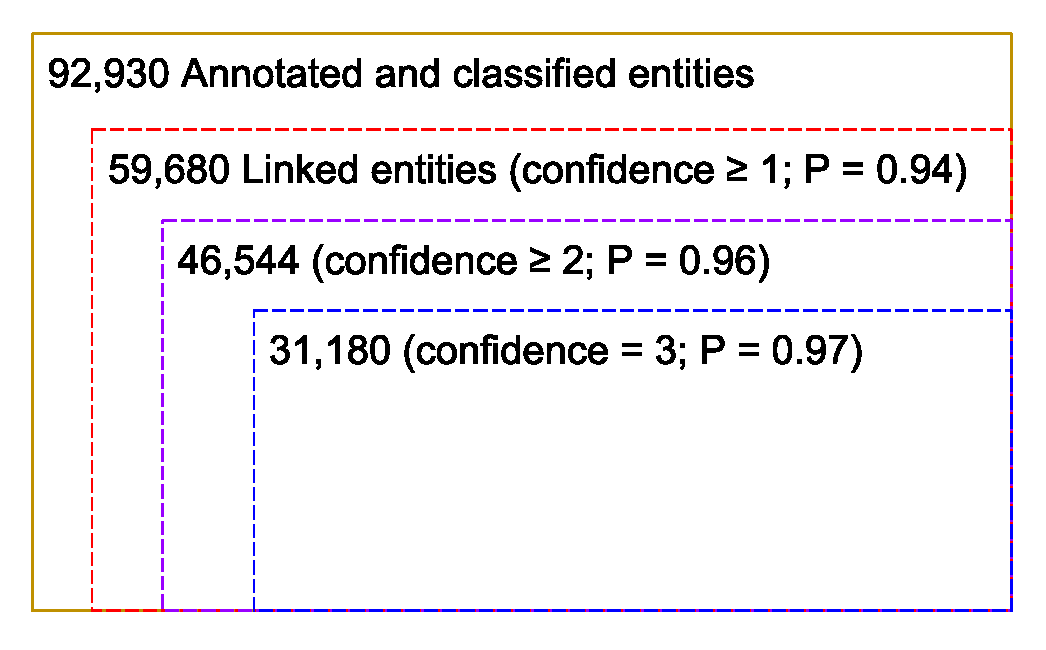
\includegraphics[width=8cm]{ch03_background/pics/ELMD_Overview.eps}
  \caption{ELMD Overview. Number of entities, confidence score and precision values in different subsets of the dataset.}
  \label{fig:elmd}
\end{figure}

\section{ELMD2}
Following the same methodology, a second set of artist biographies was gathered from Last.fm. 

From this set of documents, 200 were manually annotated by one music expert annotator. 


\section{Conclusion and Discussion}
\label{sec:elmd}

In this chapter we have described two main contributions. First, for the task of Entity Linking, we have presented an integration framework called \textsc{ELVIS} which, based on a voting procedure which leverages decisions made by an arbitrary number of off-the-shelf EL systems, provides high confident entity disambiguations. Currently, \textsc{ELVIS} incorporates three state-of-the-art systems, namely DBpedia Spotlight, Tagme and Babelfy, and can be easily extended with additional systems. The \textit{ELVIS} code is available at {\footnotesize{https://github.com/sergiooramas/elvis}}. Second, we have leveraged the potential of \textsc{ELVIS} for the creation of a novel benchmarking dataset for EL in the Music domain, called \textsc{ELMD}. This corpus comes from a collection of \textsc{Last.fm} artist biographies, and contains 47,254 sentences with 92,930 annotated and classified entity mentions (64,873 Artists, 16,302 Albums, 8,275 Songs and 3,480 Record Labels). From this set of entity mentions, 59,680 are linked to DBpedia (see Table~\ref{tbl:statistics}), with a precision of at least 0,94. In addition, by setting up a higher confidence threshold it is possible to obtain a subset of \textsc{ELMD} that prioritize higher Precision by sacrificing Recall (see Figure~\ref{fig:elmd}). The \textsc{ELMD} dataset together with the evaluation data can be downloaded from {\footnotesize{http://mtg.upf.edu/download/datasets/elmd}}.
